In the previous two sections we have discussed multiple benchmarks in two different classes: hand-written benchmarks and randomly generated benchmarks.
We have discussed the advantages and disadvantages of both.
Hand-written benchmarks cost many person-hours to write and maintain, and are usually very limited due to \ac{IP}.
Random benchmarks can overcome the scarcity of hand written ones at the cost of accuracy, they are less realistic and not as useful for assessing how well a method will perform on real use-cases.
There is a third approach that sits in-between the two above, to use machine learning to generate benchmarks with realistic properties.
This section discusses this approach and its limitations.

\subsection{Generative models}
\label{sec:generative}

\begin{figure*}[th]
	\centering
	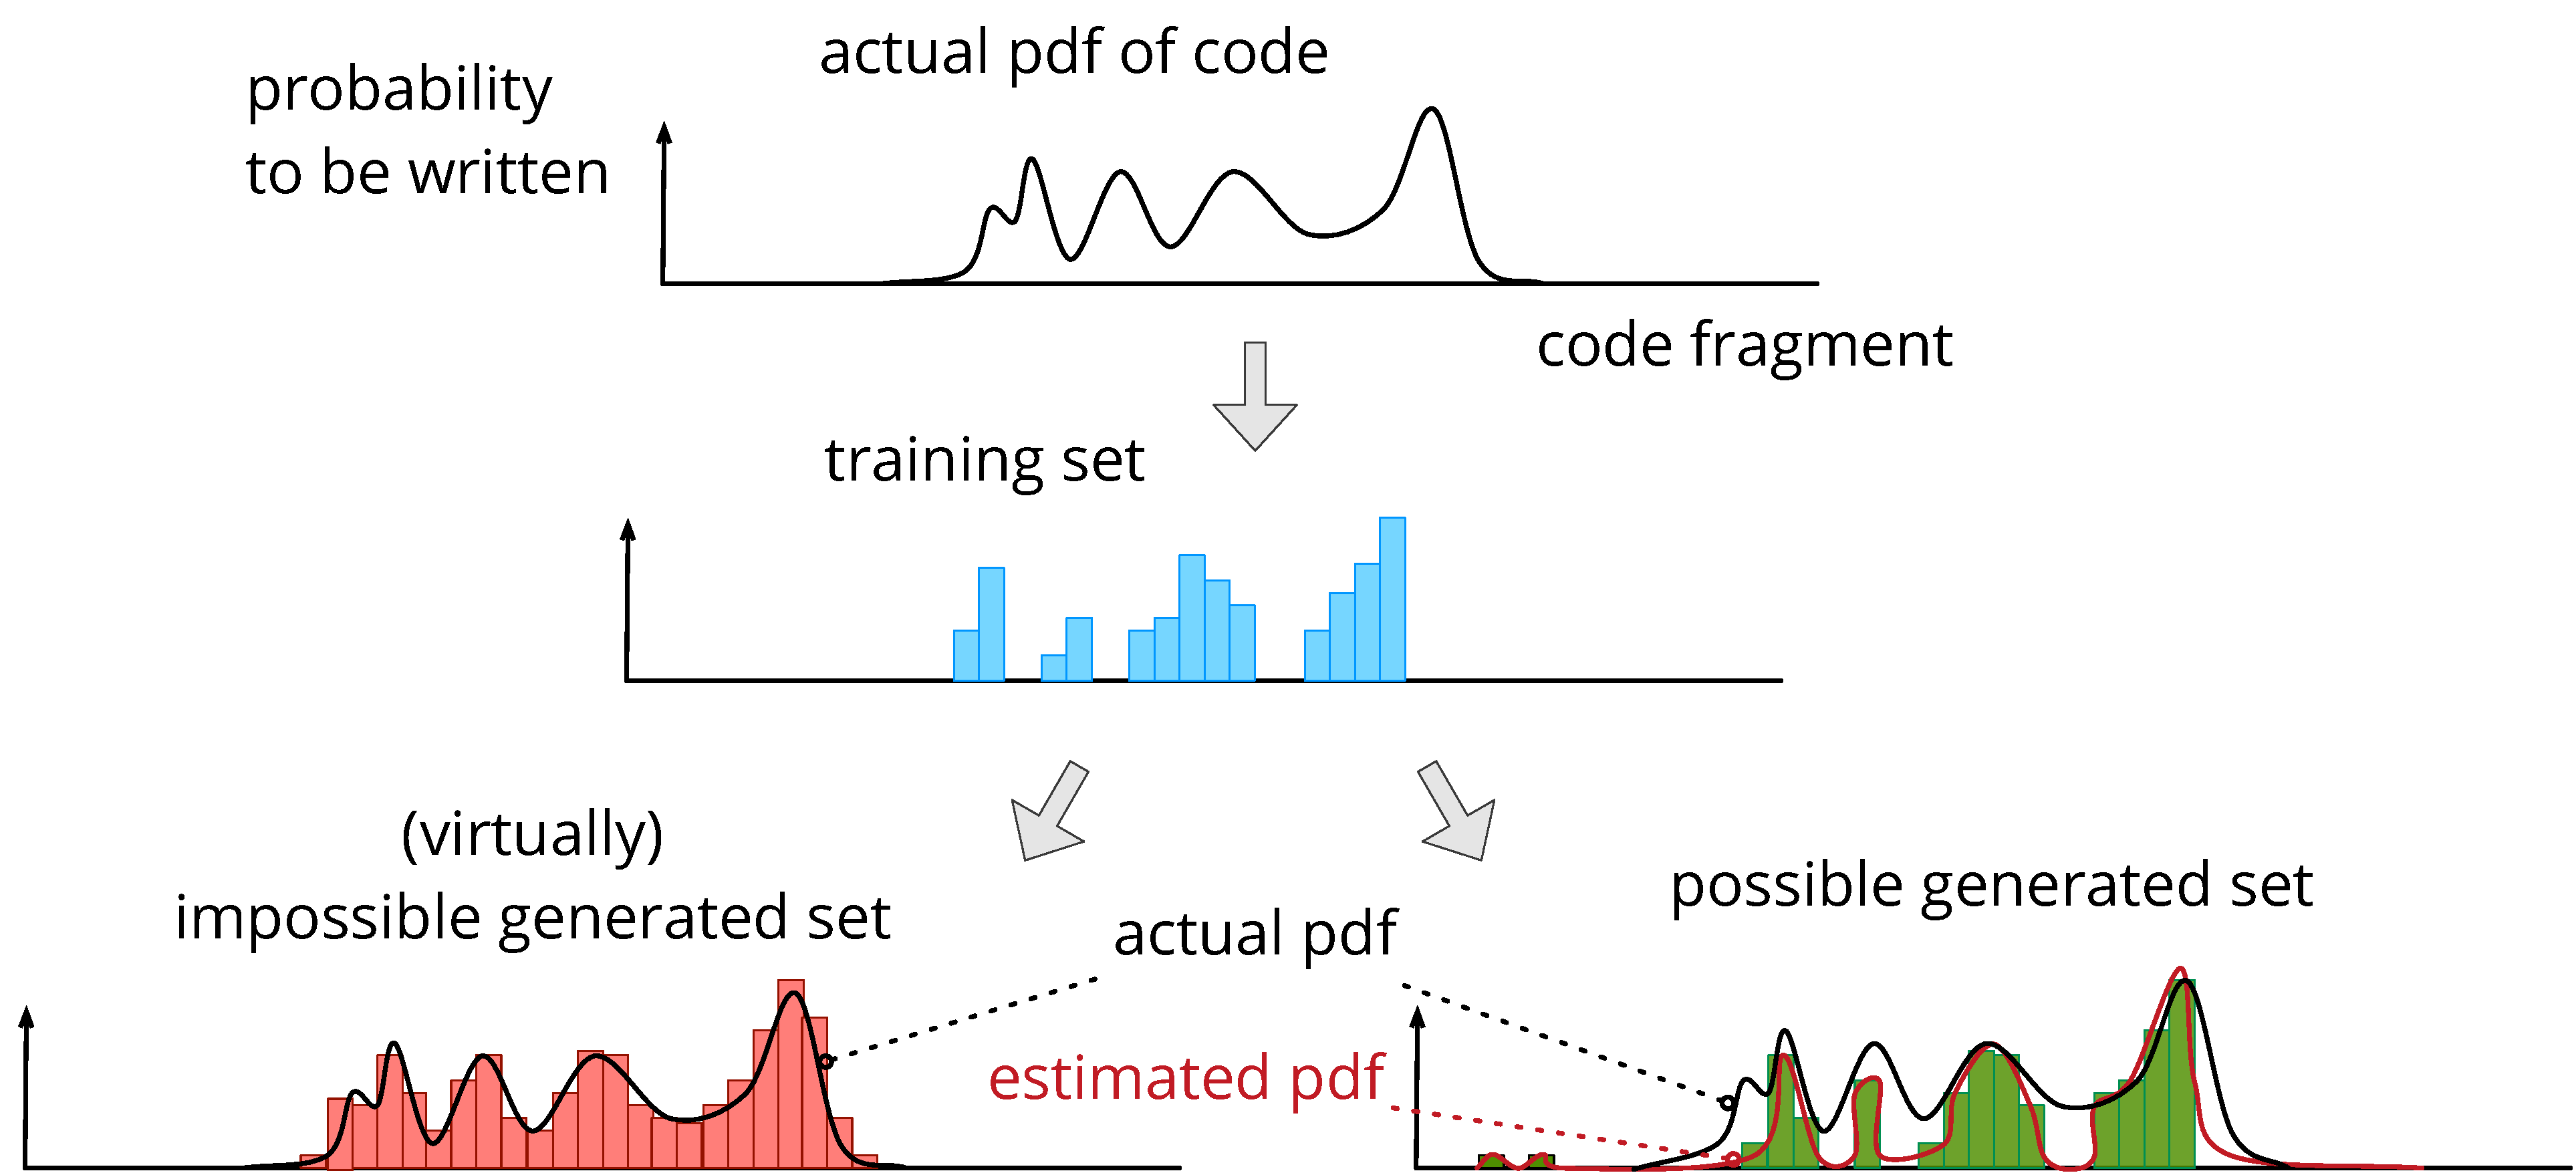
\includegraphics[width=\textwidth]{figures/illustration_histograms_ideal.pdf}
	\caption{An illustration of generative models in the Fischer-Wald setting.}
	\label{fig:histograms}
\end{figure*}

Machine learning models that could generate benchmarks fall under the general term ``generative models''.
There are different classes of generative models, however:
%Let again $p$ be the probability density function describing the probability of a programmer writing a piece of code $\omega \in \Omega$.
\begin{enumerate}
\item \label{fischer-wald} A model in the \textbf{Fischer-Wald setting} is a machine learning model solving the problem of density estimation~\cite{vapnik}. This means finding a probability $p'(t,\alpha_0)$ in a set of probabilities $\{ p'(t,\alpha) \mid \alpha \in \Lambda \}$ parametrized by elements of the parameter set $\Lambda$,
  such that for the risk functional $R(\alpha) = \int -\log(p'(t,\alpha)) dp(t)$, the value of $R(\alpha_0)$ is minimal over all $\alpha \in \Lambda$.
\item \label{conditional-estimation} A \textbf{conditional estimation} model can again mean a solution to a few different problems in different settings. For a random variable $Y$ over code, it estimates either the joint distribution $X \times Y$ or one of the conditional probabilities $p(y \mid X = x)$ or $p(x \mid Y = y)$, where $X$ is the random variable representing a piece of code (i.e. $X(\omega) = \omega$, the identity on $\Omega$)~\cite{vapnik}.

\end{enumerate}

Conditional estimation generative models have plenty of applications.
For example, conditional estimation generative models can be used for code completion tasks, which could even be leveraged to create code that is close to a specified feature vector.
With well-chosen features, this would allow for tools to create other kinds of benchmarks out of, e.g. a representative data set (see Section~\ref{sec:representative}). 
Even more so, this could be used to create domain-specific benchmarks with more samples out of a small domain-specific dataset, by producing code with feature vectors as extracted from the small dataset.
Tuning heuristics and even auto-completion tasks could all be based on conditional estimation models.
The focus of this section is the discussion of using solutions to (\ref{fischer-wald}) for benchmark generation.
This problem is the basis for generative models of code, and solutions to (\ref{conditional-estimation}) are based on or related to it as well.

\subsection{Potential Problems}
\label{sec:potential_problems}
Generative models learn to produce samples similar to those they have seen in the training data. They could then be leveraged to create arbitrarily large benchmark sets.
The problem with this is that, in the ideal case for the Fischer-Wald setting, the code produced by the generative model should be indistinguishable from the training data.
Concretely, it should be code that is also i.i.d. with respect to the (implicit) pdf of code.
If this training set is available, then it can be used instead of the synthesized benchmarks.
Figure~\ref{fig:histograms} illustrates this further.

The theoretical \ac{pdf} depicted represents, again, the probability for a particular program to be written.
To the right the illustration represents a plausible histogram of the code actually present in a training set.
Underneath it, two additional histograms are depicted. To the right, in green, a histogram that is plausibly synthesized by a good generative model trained with the training set.
While it need not be identical to the training set, it should be similar if the generative model has been trained well.
To the left, a histogram is depicted that illustrates a very implausible generated set.
How should the generative model know of the unlikely cases it has not seen, and produce no synthetic code that would never be written by a human?
By the definition in (\ref{fischer-wald}), the closer the histograms are to the depicted pdf, the better are the generative model and training set.

In case we want a ``representative benchmark'', it is thus not clear that a generative model like this is useful.
The programs created by the generative model are i.i.d. with respect to some $p'(t) = p'(t,\alpha_0)$ that is different from $p$.
For estimating $E[\mathcal{P}]$ we get additional accuracy by increasing the number of samples $l$ we use to estimate it.
This additional accuracy, however, could be canceled out by the error in $p'$ (as quantified by, e.g. $R(\alpha_0)$).
Whether this is the case, of course, depends on the concrete problem and errors, and cannot be concluded generally.
We believe, however, that it is probably the case for most instances of the state-of-the-art in generative models of code.
It is likely that with the current state of generative models, where enough training data is present to train such a model, the raw data should be at least good enough, if not even better than synthetic data from the model.

For the other kinds of benchmark, the situation is less problematic.
If we have a filter to distinguish the types of programs, e.g. one based on vectors of features interesting for the use case, then we can use generative models with these filters to produce benchmark sets of the kinds ``representative coverage benchmark'' and perhaps in some cases even ``fuzzing benchmark'', if the generative models generalize well and are run long enough to produce enough data.

\begin{figure*}[th]
	\centering
	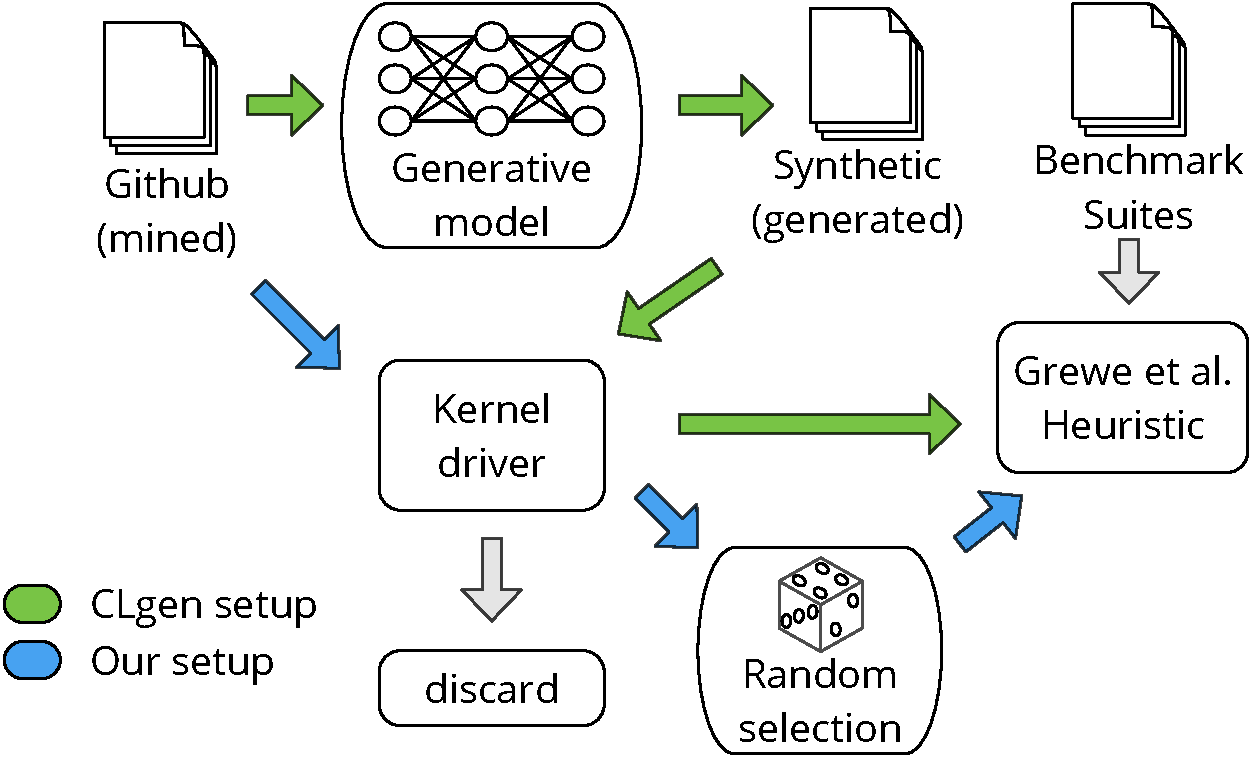
\includegraphics[width=\textwidth]{figures/clgen_flow.pdf}
	\caption{The flow of CLGen and our re-evaluation. Reproduced from Figure~1 in~\cite{goens_mapl19}.}
	\label{fig:clgen_flow}
\end{figure*}

We investigated these problems in~\cite{goens_mapl19}, where we re-evaluated the benchmark generation of CLGen~\cite{cummins_cgo17}.
Figure~\ref{fig:clgen_flow} summarizes the flow of CLGen and our re-evaluation.


\subsection{Models of Code}

Then only briefly motivate~\cite{brauckmann_cc20} and \cite{brauckmann_fdl20}.

